\documentclass[11pt]{article}

\usepackage[margin=1in]{geometry}
\usepackage{graphicx}
\usepackage{booktabs}
\usepackage{amsmath}
\usepackage{url}

\title{\textbf{Supplementary Material for LFTNet}}
\author{}
\date{}

\begin{document}

\maketitle

This supplementary material provides additional visual analyses for the
proposed LFTNet, including Local Attribution Map (LAM) analysis and qualitative
comparisons on challenging image regions. These results complement the
quantitative evaluations reported in the main paper.

% =========================================================
\section{Local Attribution Map Analysis}
% =========================================================

We further investigate the effective receptive field of different
super-resolution models using Local Attribution Maps (LAM). LAM measures the
contribution of input pixels to the reconstruction of a selected output region,
providing an intuitive visualization of the spatial information utilized by
each model.

As shown in Fig.~\ref{fig:lam}, conventional convolution-based approaches
exhibit relatively concentrated attribution regions, indicating that their
reconstruction mainly relies on local neighborhood information. In contrast,
attention-based methods generally utilize broader spatial regions.

LFTNet exhibits the widest and more distributed attribution pattern among the
compared methods. Quantitatively,LFTNet achieves a Diffusion Index (DI) of 21.90, compared with
4.07 for EDSR \cite{lim:enhanced}, 7.61 for SwinIR
\cite{liang:swinir}, 11.51 for SRFormer \cite{zhou:srformer},
and 20.89 for MambaIRv2 \cite{guo:mambairv2}. A higher DI indicates that information from a larger
spatial region contributes to the reconstruction.

These results provide additional evidence that the proposed LMSA effectively
enlarges the receptive field and facilitates long-range information interaction,
which is particularly beneficial for reconstructing complex structures and
repetitive textures.

\begin{figure}[ht]
    \centering
    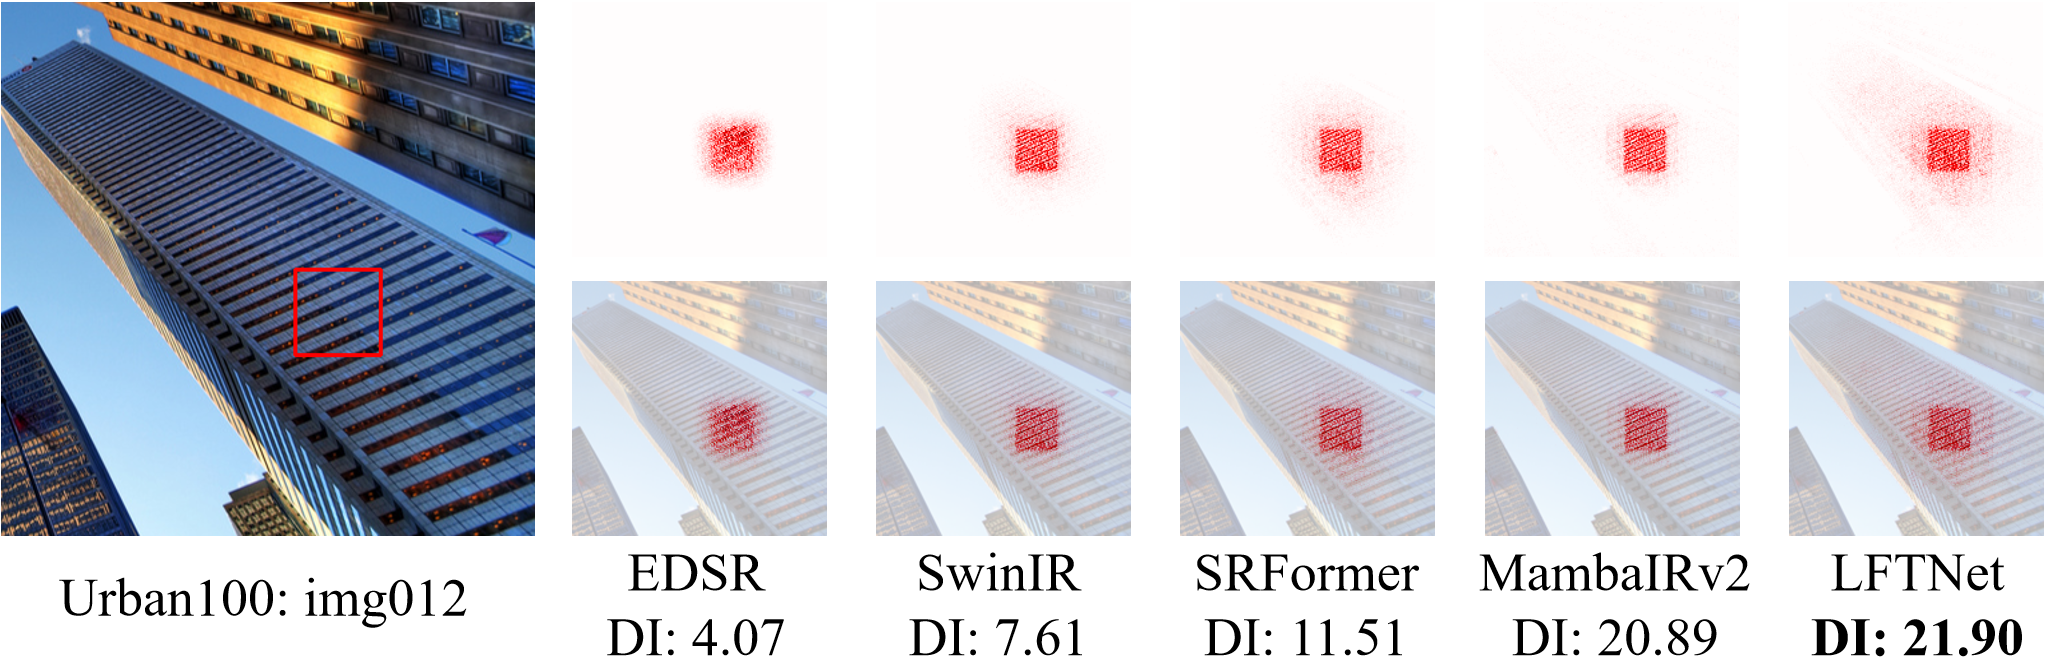
\includegraphics[width=\linewidth]{img/LAM.png}
    \caption{Local Attribution Map (LAM) comparison among different
    super-resolution methods. The Diffusion Index (DI) measures the spatial
    extent of input information involved in reconstruction.}
    \label{fig:lam}
\end{figure}


% =========================================================
\section{Qualitative Comparison}
% =========================================================

Fig.~\ref{fig:visual} presents additional qualitative comparisons on
challenging image regions containing repetitive textures, building structures,
and dense line patterns.

For building facades and stripe-like structures, bicubic interpolation and
several lightweight SR methods tend to produce over-smoothed textures,
distorted edges, or inconsistent orientations. In comparison, LFTNet better
preserves edge continuity and directional consistency, resulting in clearer
and more regular structural patterns.

For dense grids and interleaved line patterns, competing approaches may
produce broken structures, blurred boundaries, or adhesion artifacts between
adjacent lines. LFTNet reconstructs these fine structures more reliably and
maintains more regular spacing and geometric consistency, producing results
that are closer to the ground-truth HR images.

These visual comparisons further demonstrate the effectiveness of combining
long-range spatial modeling with frequency-domain feature modulation for
recovering structured and high-frequency image details.

\begin{figure}[ht]
    \centering
    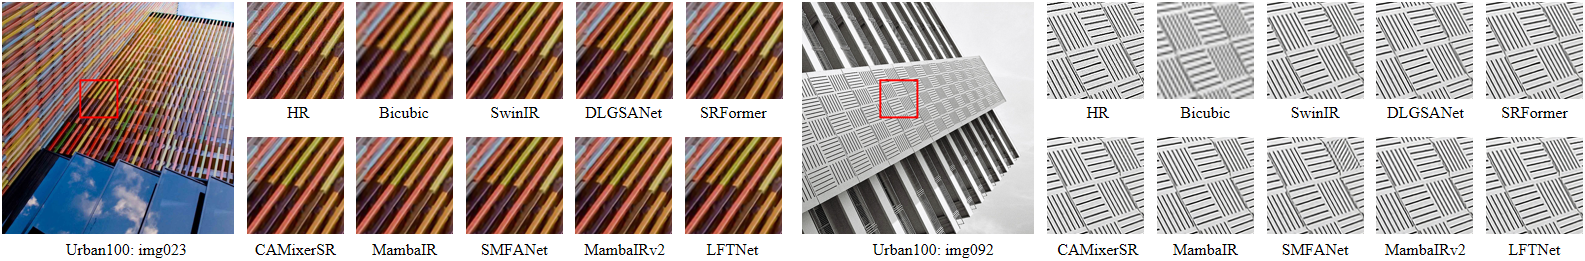
\includegraphics[width=\linewidth]{img/Vision.png}
    \caption{Additional qualitative comparisons of lightweight image
    super-resolution methods on challenging image regions.}
    \label{fig:visual}
\end{figure}


% =========================================================
\section{Discussion}
% =========================================================

The LAM and qualitative results provide complementary evidence to the
quantitative evaluations in the main paper. LMSA enables the model to exploit
a broader spatial context through direction-complementary long-range
interaction, while FGFN enhances informative structural and texture components
through frequency-selective modulation. Their combination improves the
reconstruction of both large-scale structures and fine repetitive details
under a lightweight model budget.
\bibliographystyle{IEEEtran}
\bibliography{refs}
\end{document}


